% !TEX encoding = UTF-8 Unicode

\chapter{Tworzenie zbiorów danych}
Priorytetem było stworzenie zestawu danych
umożliwiającego rozwój różnych modeli sieci neuronowych bez konieczności każdorazowego
ingerowania w zbiór lub dopasowywania go specjalnie do konkretnej sieci.\\
\textbf{Wszystkie zbiory dostępne są pod linkami w części Dodatek A [\ref{dodatekA}] }

\section{Zbiór obrazów kwadratowych}
Pierwszym założeniem było zrobienie określonej ilości zdjęć kości położonej na środku
obrazu otrzymywanego z kamery, na obszarze kwadratu o boku około 3 krotnie większym
niż długość ściany samej kości. Miało to umożliwić kadrowanie obrazów
do niewielkich rozmiarów z kośćmi położonymi w różnych jego miejscach.\\
Kolejną kwestią była konieczność przystosowania sieci do rozpoznawania kości o
różnych kolorach ścian, oczek i samego tła. Ponieważ docelowo sieć
miała operować na rzeczywistym obrazie z kamery, ważne było także zapewnienie poprawnego
działania w przypadku niewielkich zniekształceń obrazu bądź szumów.\\
Powyższe wymagania narzuciły konkretną formę zestawów danych.
Każdy zestaw ma ustaloną barwę tła, kości oraz oczek. Każda ścianka sfotografowana jest
od 3 do 30 razy, określając liczebność każdego ze zbiorów miedzy 18 a 180 zdjęć.
Zdjęcia w niektórych zestawach poddawane były działaniu lub ostrego punktowego światła
w celu wygenerowania trudniejszych do rozpoznania obrazów. Poszczególne zestawienia
kolorystyczne w tych zbiorach wypisane są w tabeli poniżej. \newpage

\begin{table}[ht]
\centering
\begin{tabular}{rcl|cc}
 \multicolumn{3}{c}{Kolor} & \multicolumn{2}{c}{Ilość zdjęć} \\ \hline
kości & oczek & tła & ściany & kostki \\ \hline
biały & czarny & czerwony & 30 & 180 \\
biały & czarny & granatowy & 3 & 18 \\
biały & czarny & czarny & 8 & 48 \\
beżowy & czarny & czerwony & 3 & 18 \\
czarny & biały & czarny & 10 & 60 \\
czarny & biały & czerwony & 10 & 60 \\
czerwony & biały & czerwony & 5 & 30 \\
czerwony & czarny & czerwony & 3 & 18 \\
granatowy & złoty & biały & 4 & 24 \\
granatowy & złoty & niebieski & 6 & 36 \\
zielony & biały & zielony & 8 & 48 \\
zielony & biały & biały & 5 & 30 \\
różowoczerwony & czarny & biały & 5 & 30 \\ \hline
\multicolumn{3}{c}{\textit{Łączna ilość zdjęć:}} & \textit{100} & \textit{600}
\end{tabular}
\vspace{0.2cm}
\caption{Zestawienie kolorystyczne obrazów 1}
\label{tab:zestawienie1}
\end{table}

Każdy z obrazów został następnie poddany przekształceniom by zwiększyć ich ilość, konieczną
do prawidłowego uczenia się sieci. Miało to także zapewnić zniekształcone w niewielkim stopniu
zdjęcia, które również powinny być rozpoznawane przez sieć. W tym przypadku zastosowano sześć
takich przekształceń. \\
Następnym krokiem było zastosowanie obrotów o kąty 5\textsuperscript{o},
15\textsuperscript{o}, 30\textsuperscript{o} lub 45\textsuperscript{o}, w celu dobrania
najbardziej adekwatnej ilości obrazów do rozmiaru sieci oraz ilości parametrów
do nauczenia się. Po wielu próbach ostatecznie wybrano kąt 15\textsuperscript{o}, zapewniający
wystarczająco liczny zbiór treningowy do możliwości uczenia sieci oraz nie
wydlużało znacząco czasu potrzebnego do przetworzenia wszystkich obrazów.\\
Powyższe procesy spowodowały uzyskanie 168 zdjęć o rozmiarze 64x64 piksele z każdego
z początkowych obrazów o rozmiarze 1600x1200 pikseli. Cały zbiór danych liczył 100800
obrazów, zarówno w wersji kolorowej RGB oraz w odcieniach skali szarości. Części
treningowa i testowa zbioru danych zostały rozdzielone w stosunku 4:1, dając odpowiednio
80640 oraz 20160 zdjęć w każdym z nich. \\\\

\begin{figure}[h]
\centering
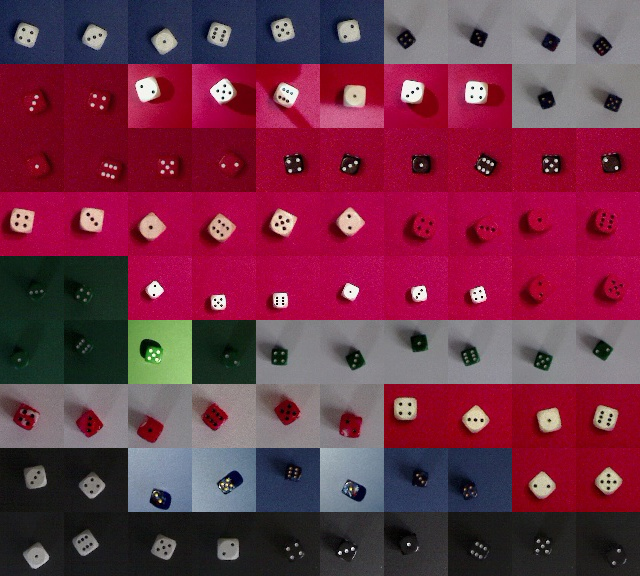
\includegraphics[scale=0.35]{images/kolaz}
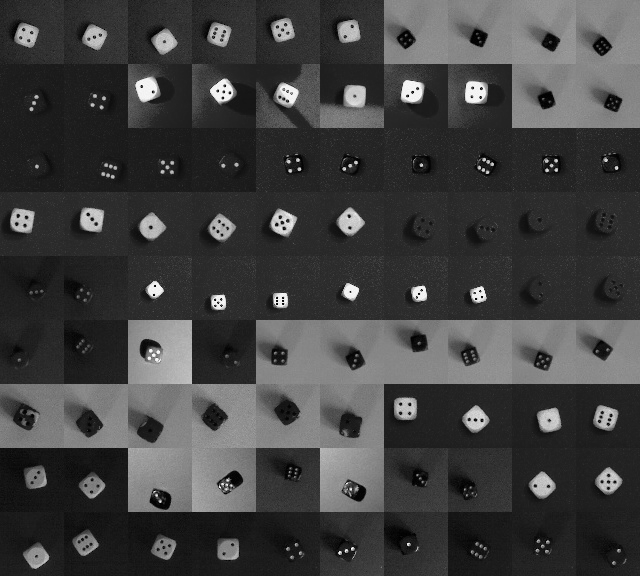
\includegraphics[scale=0.35]{images/kolaz_grayscale}
\caption{Obrazy o rozdzielczościach 64x64}
\end{figure}

Nieocenioną pomocą w początkowej fazie prac nad tworzeniem i uczeniem sieci neuronowych
z obrazami w kształcie kwadratów był fakt, że praktycznie wszystkie przykłady dostępne
w opracowaniach naukowych korzystały ze zdjęć w tym kształcie. Również wszystkie
przykłady opisane w różnych poradnikach czy najpopularniejsze zbiory jak MNIST oraz
CIFAR10 zawierają kwadratowe obrazy. Przyjęcie takiego kształtu ułatwiło dobór parametrów
sieci, nie narzucając osobnych wartości w poziomie i pionie.

 \section{Zbiór obrazów prostokątnych}

Po nauczeniu i weryfikacji kilkunastu różnych modeli sieci, zdecydowano się podjąć
próbę z wykorzystaniem większych obrazów oraz kości rozmieszczonych w miejscach
bardziej zróżnicowanych niż jedynie pewien, niewielki obszar w centrum obrazu.
Kolejne zdjęcia miały również podnieść trudność uczenia poprzez zmniejszenie
rozmiaru kości w stosunku do rozmiaru całego obrazu. Ostatnim czynnikiem decydującym o
rozwinięciu zbiorów danych była trudność w rozpoznawaniu kości w czasie rzeczywistym
w sytuacji kiedy rozmiar obrazu lub jego wycinka to jedynie 64x64 piksele. Zwiększenie
rozmiarów ułatwiłoby identyfikacje kości oraz umożliwiło by detekcję ilości oczek
wyrzuconych na kostce o ile tylko kość znalazła by się w obszarze odejmowanym przez kamerę. \\
Plan zakładał wykorzystanie poprzednio wykonanych zdjęć oraz dodanie nowych
z kośćmi rozmieszczonymi poza obszarem w centrum obrazu w celu rozwinięcia możliwości sieci.
Jednocześnie zrodził się pomysł wykorzystania prostokątnych obrazów, które lepiej oddawałyby
rzeczywistość, gdzie prawie wszystkie kamery, niezależnie od zastosowań, dostarczają
prostokątny obraz. W tym celu, analogicznie jak w przypadku kwadratowych obrazów,
zostały wykonane zdjęcia o określonych zestawieniach kolorystycznych. W tabeli poniżej
wypisane jest ich zestawienie:

\begin{table}[h!]
\centering
\begin{tabular}{rcl|cc}
 \multicolumn{3}{c}{Kolor} & \multicolumn{2}{c}{Ilość zdjęć} \\ \hline
kości & oczek & tła & ściany & kostki \\ \hline
biały & czarny & zielony & 6 & 36 \\
czerwony & biały & zielony & 6 & 36 \\
czerwony & czarny & różowy & 7 & 42 \\
czarny & biały & szary & 6 & 36 \\
czarny & biały & niebieski & 6 & 36 \\
beżowy & czarny & szary & 6 & 36 \\
beżowy & czarny & niebieski & 6 & 36 \\
granatowy & złoty & biały & 8 & 48 \\
zielony & biały & żółty & 7 & 42 \\
różowoczerwony & czarny & pomarańczowy & 6 & 36 \\ \hline
\multicolumn{3}{c}{\textit{Łączna ilość zdjęć:}} & \textit{64} & \textit{384}
\end{tabular}
\vspace{0.2cm}
\caption{Zestawienie kolorystyczne obrazów 2}
\label{tab:zestawienie2}
\end{table}

\begin{figure}[h]
\centering
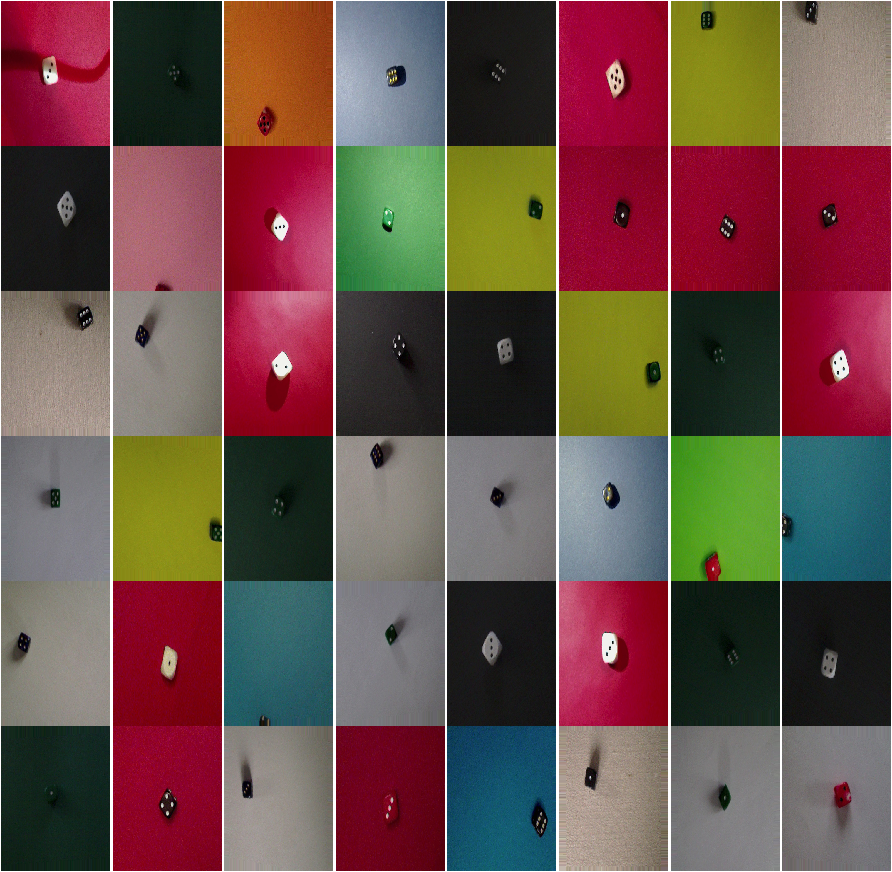
\includegraphics[scale=0.5]{color_dices}
\caption{Obrazy o rozdzielczościach 106x79}
\end{figure}

Ilość zdjęć prostokątnych jest mniejsza niż kwadratowych z powodu czasu jaki zajmuje
wykonanie takiej ilości zdjęć oraz chęć wykorzystania obu rodzajów zbiorów do uczenia sieci.
Powstała w ten sposób liczba 984 unikalnych zdjęć jest wystarczająca do realizacji
zamierzonego zadania i pozwala na odpowiednie uczenie sieci. \\
Poprzednio wykorzystywane obrazy, miały wymiary 64x64 piksele co łącznie odpowiadało
4096 lub 12288 wartościom pikseli odpowiednio dla obrazów w skali szarości oraz
kolorowych RGB. Nowo utworzony zbiór obrazów prostokątnych w pierwszym założeniu miał
składać się z obrazów o rozmiarach 320x240 pikseli w skali szarości, co oznaczało
76800 wartości na jedno zdjęcie. W wyniku niepowodzenia procesu uczenia po kilku godzinach,
podjęto decyzję o dwukrotnym zmniejszeniu obrazów do 160x120 pikseli. Wartość ta
została wybrana ponieważ ilość parametrów obrazu, wynosząca 19200, była jedynie o 56\%
większa od ich liczby dla kolorwych obrazów 64x64. Próby uczenia się sieci pokazały jednak,
że lepszym rozwiązaniem będzie zastosowanie mniejszych o 50\% obrazów o wymiarach
106x79 pikseli co skutkuje liczbą 8374 wartości na jeden obraz.\\
Wraz z problemami związanymi z rozmiarami obrazów, zdecydowano się na zmniejszenie ilości
przekształceń z sześciu do wybranych czterech, najbardziej efektowych. Inne przedstawiały
zmieniony w niewielkim stopniu obraz, niepotrzebnie wydłużając proces
uczenia. Również kąt obrotu zdjęć został zwiększony z 15\textsuperscript{o}
do 30\textsuperscript{o}, co w założeniu nie powinno powodować problemów z rozpoznawaniem
kości przy różnych ustawieniach. \\
Wszystkie operacje umożliwiły osiągnięcie 60 obrazów z każdego początkowego zdjęcia, w rozmiarze
106x79 pikseli w odcieniach skali szarości. Całkowita ilość obrazów w pełnym zbiorze
danych wynosiła 59040, co przełożyło się na 47232 obrazów treningowych i 11808 testowych,
korzystając z identycznego jak wcześniej stosunku 4:1.
